% ============================================================================
% MedVisionQuery — revised report sections (October 2026)
% Drop-in replacements for the NeurIPS-template report (Group 9).
% Requires: \usepackage{booktabs}, \usepackage{graphicx} (already in the NeurIPS template setup).
% Figure: copy system_diagram.png from the repo root next to the .tex file.
% Numbers are from the 200-case evaluation committed at c30e161 (see README).
% ============================================================================

% ----------------------------------------------------------------------------
% ABSTRACT (replace)
% ----------------------------------------------------------------------------
\begin{abstract}
Medical visual question answering (VQA) over radiology images combines perception, question interpretation,
answer synthesis and verification---steps that fail in different ways and are hidden inside a single model call.
We present MedVisionQuery, an agentic system in which a Haystack Agent controller decides, case by case, how to
look at the image, answer, verify the answer \emph{against the image}, and whether to re-examine a specific region,
revise, abstain or finish. Perception is question-aware, the answerer and the verifier both see the image, and a
different, larger model verifies. We evaluate on 200 randomly sampled VQA-RAD test questions against a single-prompt
baseline, a hand-designed workflow and a fixed-pipeline ablation, all on the same answering model, scoring with a
strict rule-based scorer and a blinded LLM judge. The agentic loop matches the single prompt in accuracy
(64.5\% vs.\ 63.5\% strict; 72.0\% vs.\ 70.0\% judged; McNemar $p=0.86$), clearly beats the fixed pipeline
(+7.5 points, $p=0.02$) and the workflow (28.0\%), and is substantially more reliable: its verification and
self-consistency signals predict errors, it abstains on hard cases, and only 2\% of its answers change across
re-runs versus 12\% for the single prompt---at about 45$\times$ the cost. Code:
\url{https://github.com/clarence-ck/med-vqa-rad-agentic}.
\end{abstract}

% ----------------------------------------------------------------------------
% SECTION 1 (edit the last paragraph only)
% ----------------------------------------------------------------------------
% Replace the final paragraph of Section 1 with:
We target the VQA-RAD benchmark~\cite{lau2018vqarad}: 2,244 image--question pairs in the Hugging Face release
(1,793 train / 451 test), with close-ended and open-ended questions. We evaluate on a seeded random sample of 200
test questions; no training data is used.

% ----------------------------------------------------------------------------
\section{Agent Architecture}
% ----------------------------------------------------------------------------
\begin{figure}[t]
  \centering
  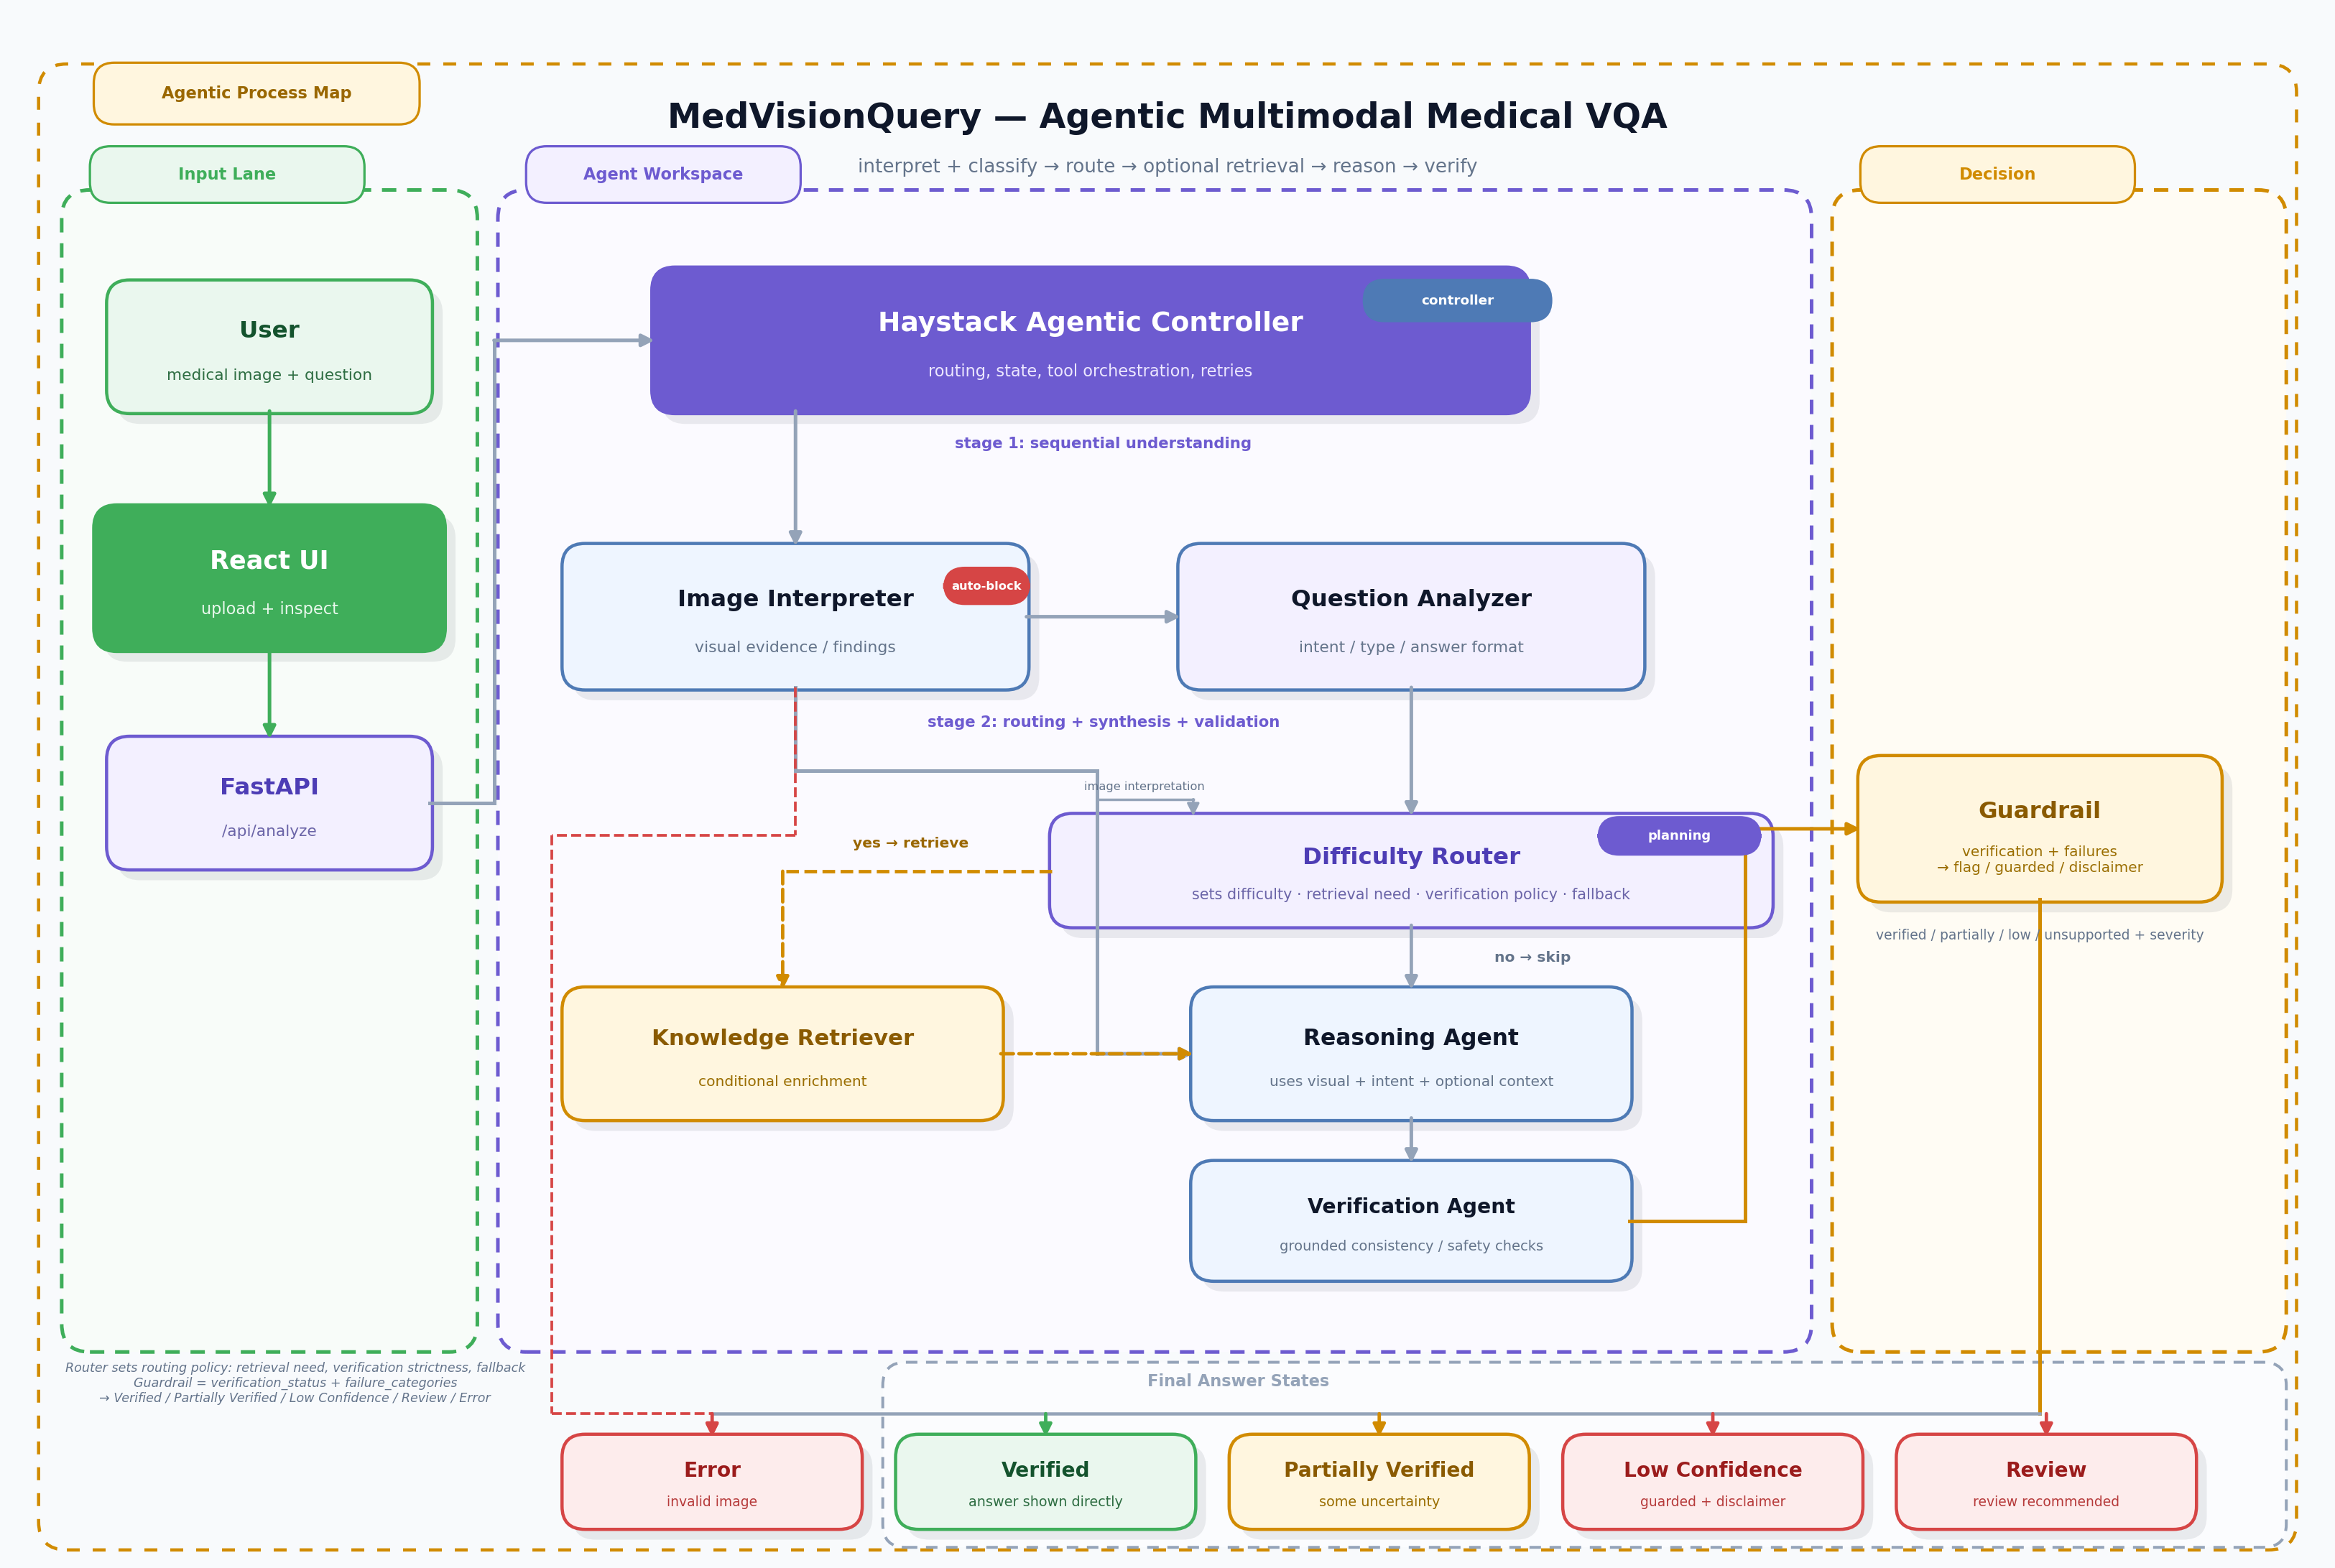
\includegraphics[width=\linewidth]{system_diagram.png}
  \caption{MedVisionQuery. A Haystack Agent controller calls question analysis, question-aware perception
  (\texttt{look}), answer synthesis and image-grounded verification (\texttt{check}); \texttt{check}'s recommendation
  drives a focused re-look, a revised answer, abstention or finish. A decision-and-safety stage keeps the
  best-verified answer, measures self-consistency and applies guardrails.}
  \label{fig:arch}
\end{figure}

\paragraph{Controller loop.} A fresh Haystack \texttt{Agent} is created per request (Figure~\ref{fig:arch}). Its
five tools are bound to per-request working memory holding the image, the question analysis, and every look,
answer and check; the controller sees only short text results and chooses the next call. Unlike our earlier
fixed pipeline, the tool sequence depends on what verification finds: on the 200 evaluation cases the controller
finished directly in 141 cases, re-examined a region in 19, revised its answer in 29 and abstained in 11. Budgets
cap the loop at two focused re-looks, three answers and 16 steps, with a safety net that checks the latest answer
if the controller stalls.

\paragraph{Roles.}
\textbf{\texttt{analyze\_question}} (planner input) classifies the question type and expected answer format.
\textbf{\texttt{look(focus)}} (perception) examines the image \emph{with the question in mind}; with a focus, it
re-examines a named region; the first look rejects non-radiology images.
\textbf{\texttt{answer(guidance)}} (executor) answers from the image plus all observations, applying the
verifier's guidance on revisions.
\textbf{\texttt{check}} (evaluator) verifies the answer against the image with five checks, returns a status
(verified, partially verified, low confidence, unsupported) and recommends \emph{accept}, \emph{relook} with a
focus, \emph{reanswer} with guidance, or \emph{abstain}.
\textbf{\texttt{finish(abstain)}} ends the episode and is refused while the latest answer is unchecked.

\paragraph{Model and tool choices.} All roles use OpenAI models, sized by need and configurable per role. The
controller and question analysis make simple decisions (\texttt{gpt-6-luna}, no/low reasoning effort); perception
and answering use \texttt{gpt-6-luna} with medium effort, after a pilot showed that giving the answerer the image
mattered far more than model size (50\%$\to$70\% on 20 cases). Verification uses a different, larger model
(\texttt{gpt-6.1-sol}) so that the answering model does not verify itself. Haystack's \texttt{Agent}/\texttt{Tool}
abstraction provides the tool-calling loop and exit conditions; keeping the image in per-request memory rather than
in the controller's context keeps the controller cheap. An earlier retrieval stage over SLAKE was removed: it
returned other patients' question--answer pairs, which contradicted yes/no and location answers and gave no
measurable benefit on perception-bound questions.

\paragraph{Baselines and ablation.} The \emph{single-shot baseline} sends the image and question in one prompt. The
\emph{workflow baseline} is a fixed chain---a question-agnostic image description, question analysis, then
hand-written rules per question type. The \emph{fixed-pipeline ablation} runs our original six stages (interpret,
analyse, filter, route, reason, verify, with retry) in a fixed order with the image given to the reasoner, isolating
what the controller's decisions add. A demo UI (Dashboard, Case Explorer, Evaluation; Section~\ref{sec:ui}) exposes
all systems.

% ----------------------------------------------------------------------------
\section{Multimodal Grounding}
% ----------------------------------------------------------------------------
The system uses two modalities, the radiology image and the text question, and they interact at every step that
determines the answer: the question (and any focus) steers what \texttt{look} examines; \texttt{answer} and
\texttt{check} receive the image directly alongside the text observations; only the controller works purely in
text. Our earlier design described the image once, \emph{without} the question, and passed only that text downstream;
in a 20-case pilot all four failures of that design were ``cannot be determined from the image description'', and
all four were answered correctly once the reasoner saw the image. Because the verifier sees the image, its
``explanation grounded in evidence'' and ``no contradictions'' checks are genuine cross-modal agreement checks.

% ----------------------------------------------------------------------------
\section{Control and Failure Handling}
% ----------------------------------------------------------------------------
\textbf{Detection.} Image-grounded verification (five checks and a status), seven failure categories
(\emph{unsupported claim}, \emph{low confidence}, \emph{visual contradiction}, \emph{partially verified},
\emph{question--answer mismatch}, \emph{generation unstable}, \emph{parser failure}) and an eighth,
\emph{self-inconsistent}, from resampling.
\textbf{Recovery.} Instead of re-running the whole pipeline, the controller re-examines the region the verifier
names or revises the answer with the verifier's guidance. A later answer replaces an earlier one only if its check
is strictly better, because focused re-looks can over-read.
\textbf{Self-critique.} After finishing, the answerer is re-asked independently twice; low agreement adds a failure
category and flags the case for review.
\textbf{Fallback.} The controller may abstain (reported as an abstention, never coerced into ``no''); a guardrail
adds a disclaimer and a review flag for low-confidence, unsupported, high-severity or self-inconsistent cases;
non-radiology or unreadable images are rejected before any answer is produced.

% ----------------------------------------------------------------------------
\section{Evaluation}
% ----------------------------------------------------------------------------
\paragraph{Setup.} 200 VQA-RAD test questions drawn at random (seed 42; 111 close-ended, 89 open-ended); all four
systems run on the same cases with the same answering model. \emph{Strict scoring}: yes/no answers must start with
the correct word; binary terms must name the correct term and not its opposite; counts must match; open-ended answers
must contain every content word of the reference (aliases and plurals folded; $\geq$60\% for references longer than
three words), with left/right conflicts and denials counted wrong and embedding similarity only as a strict
fallback. Because strict scoring rejects correct paraphrases, a \emph{blinded LLM judge} (\texttt{gpt-6.1-sol},
answers shuffled and anonymised) re-assesses strict-wrong open-ended answers; a 30-verdict spot check agreed on 29/30
credit decisions. Paired comparisons use the exact McNemar test; 95\% intervals are about $\pm$6.7 points. The
baseline and agentic loop were re-run on 50 cases to measure stability. API cost of the evaluation (runs, repeats and judge): \$4.06.

\begin{table}[t]
  \centering
  \caption{Accuracy on 200 random VQA-RAD test questions (same answering model for all systems).}
  \label{tab:main}
  \small
  \begin{tabular}{lcccccc}
    \toprule
    System & Strict & Judged & Close (111) & Open (89) strict/judged & Time & Cost \\
    \midrule
    Single-shot baseline      & 63.5 & 70.0 & 76.6 & 47.2 / 61.8 & 4.4\,s  & \$0.0002 \\
    Workflow baseline         & 28.0 & 31.0 & 42.3 & 10.1 / 16.9 & 9.0\,s  & \$0.0005 \\
    \textbf{Agentic loop}     & \textbf{64.5} & \textbf{72.0} & 76.6 & 49.4 / 66.3 & 37.2\,s & \$0.0094 \\
    Fixed pipeline (ablation) & 57.0 & 61.5 & 68.5 & 42.7 / 52.8 & 38.1\,s & \$0.0070 \\
    \bottomrule
  \end{tabular}
\end{table}

\paragraph{Results.} Table~\ref{tab:main}. The agentic loop and the single prompt are statistically
indistinguishable (17 vs.\ 15 discordant cases, $p=0.86$; judged $p=0.61$). The controller's decisions clearly help
relative to the same models in a fixed order (26 vs.\ 11, $p=0.02$; judged 32 vs.\ 11, $p=0.002$), and both far
exceed the hand-designed workflow. Gains concentrate where the controller acts: on cases it re-examined it scored
47\% versus 37\% for the single prompt, and on revised cases 55\% versus 45\% (Table~\ref{tab:paths}).

\begin{table}[t]
  \centering
  \caption{Accuracy (strict, \%) by the path the controller took, and agentic accuracy by its own signals.}
  \label{tab:paths}
  \small
  \begin{tabular}{lcccc@{\hskip 18pt}lc}
    \toprule
    Path & $n$ & Agentic & Single & Pipeline & Signal & Agentic \\
    \midrule
    direct    & 141 & 74 & 72 & 67 & verified (169)            & 70 \\
    relook    & 19  & 47 & 37 & 37 & partially verified (25)   & 40 \\
    reanswer  & 29  & 55 & 45 & 31 & unsupported/low (6)       & 0  \\
    abstained & 11  & -- & 45 & 36 & consistency high (162)    & 72 \\
              &     &    &    &    & consistency med/low (27)  & 40--53 \\
    \bottomrule
  \end{tabular}
\end{table}

\paragraph{Failure case analysis.}
\emph{Self-consistency:} two independent re-answers per case; high consistency means 72\% accuracy, medium/low
40--53\%, so low consistency marks uncertainty rather than certain error.
\emph{Cross-modal agreement:} because the verifier sees the image, verification status is predictive: verified
answers are 70\% correct, unsupported or low-confidence answers 0\%.
\emph{Verifier model:} a larger model verifying a smaller one steers 59 of 200 episodes away from the direct path.
\emph{Disagreement:} the three systems disagree on 65\% of cases; when exactly one system is right, it is the agentic
loop 16 times, the single prompt 12 and the workflow 7.
\emph{Stability:} on 50 repeated cases, 12\% of single-prompt answers flipped between right and wrong, versus 2\% for
the agentic loop.
Four patterns dominate the errors: (i) a shared perception blind spot, where looker and verifier misread the image the
same way (e.g.\ bowel gas read as free air after two focused re-looks); (ii) over-reading on re-looks, limited by
keeping the best-verified answer; (iii) benchmark items whose question does not match the image, which every system
fails; and (iv) workflow rigidity, where fixed rules answer ``Brain'' or ``X-ray'' when a specific finding is needed.

% ----------------------------------------------------------------------------
\section{User Interface}\label{sec:ui}
% ----------------------------------------------------------------------------
A React frontend exposes three views: \textbf{Dashboard} (upload an image, compare the agentic loop with both
baselines, inspect the trace, verification checks and failure categories), \textbf{Case Explorer} (browse the 200
evaluation cases with full agent traces) and \textbf{Evaluation} (strict and judged accuracy for all four systems,
accuracy by question type and by controller path, disagreement and a per-case table).

% ----------------------------------------------------------------------------
\section{Reflection}
% ----------------------------------------------------------------------------
\paragraph{When agentic behaviour is beneficial.} Not for raw accuracy on this benchmark: a strong single prompt on
the same model is as accurate. The agentic system pays off when answers must be \emph{trustworthy}: its
verification and consistency signals identify likely errors, it abstains on cases where the single prompt is wrong
more often than right, it recovers on hard cases by re-examining specific regions, its answers are far more stable
across runs, and every decision is auditable. Against a fixed multi-stage pipeline with identical models, letting a
controller decide is clearly better---the benefit comes from \emph{adaptive control}, not from decomposition alone.

\paragraph{Limitations.} About 45$\times$ the cost and 8$\times$ the latency of a single prompt for equal accuracy.
The verifier shares the perception weaknesses of vision models, so agreement is not correctness. Two hundred cases
give $\pm$6.7-point intervals and noisy per-type estimates; the LLM judge is an upper bound, spot-checked but not
human-annotated. A retrieval stage did not help perception-bound questions and was removed; retrieval may still
help questions that need knowledge not visible in the image, which VQA-RAD rarely contains.
